\documentclass[a4paper, 12pt]{article}

\usepackage{graphicx}
\usepackage{subcaption}
\usepackage{amsmath}
\usepackage{url}
\usepackage{tikz}
\usepackage{siunitx}

\let\vec\mathbf  % Make vectors bold, instead of arrow

\newcommand\beq{\begin{equation}}
\newcommand\eeq{\end{equation}}
\newcommand{\del}[2]{\frac{\partial #1}{\partial #2}}

\author{Thorvald M. Ballestad}
\title{Assignment 2 - TFY4235\\
  Biased brownian motion}

\begin{document}
\maketitle

\textbf{Task 1}

Euler scheme
\beq\label{eq:euler}
x_{n+1} = x_n - \frac1\gamma_i \del{U}{x} \delta t + \sqrt{\frac{2k_B T\delta t}{\gamma_i}} \hat{\xi_n}.
\eeq

Introducing
\beq
\hat{x} = \frac{x}{L},\quad
\hat{t} = \omega t,\quad
\omega = \frac{\Delta U}{\gamma_i L^2},\quad
\hat{U}(\hat{x}, \hat{t}) = \frac{U(x, t)}{\Delta U},\quad
\hat{D} = \frac{k_BT}{\Delta U},
\eeq

\eqref{eq:euler} can be rewritten as
\beq
\hat{x}_{n+1} = \hat{x}_n - \del{\hat{U}}{\hat{x}}(\hat{x}, \hat{t})\delta \hat{t} + \sqrt{2\hat{D}\delta\hat{t}} \hat{\xi}_n.
\eeq

Here $\hat{U} = \hat{U}_r(\hat{x}) f(\hat{t})$ where
\begin{equation}
  \hat{U}_r(\hat{x}) =
  \begin{cases}
    \frac{\hat{x}}{\alpha}, &\quad \text{ if } 0 \leq \hat{x} < \alpha\\
    \frac{1-\hat{x}}{1-\alpha}, &\quad \text{ if } \alpha \leq \hat{x} < 1
  \end{cases},
  \quad
  f(\hat{t}) =
  \begin{cases}
    0 &\quad \text{ if } 0\leq \hat{t} < \frac{3\omega\tau}{4}\\
    1 &\quad \text{ if } \frac{3\omega\tau}{4} \leq \hat{t} < \omega\tau
  \end{cases}.
\end{equation}

The criterion for $\delta t$ in dimensionless quantities become
\beq
\operatorname{max} \left| \del{\hat{U}}{\hat{x}}\right| \delta \hat{t}
+ 4\sqrt{2\hat{D} \delta\hat{t}} \ll \alpha
\eeq

\textbf{Task 7}

The Boltzmann distribution
\beq
p(U) =
\frac{
  e^{-\frac{U}{k_BT}}
}{
  k_BT \left(
  1 - e^{-\frac{\Delta U}{k_BT}}
  \right)
}.
\eeq
Which, in dimensionless quantities is
\beq
p(\hat{U}) =
\frac{
  e^{-\hat{U}/\hat{D}}
}{
  \hat{D} \left(
  1 - e^{-1/\hat{D}}
  \right)
}.
\eeq

\begin{figure}[h]
  \centering
  \subcaptionbox{$D=\frac{1}{10}$}{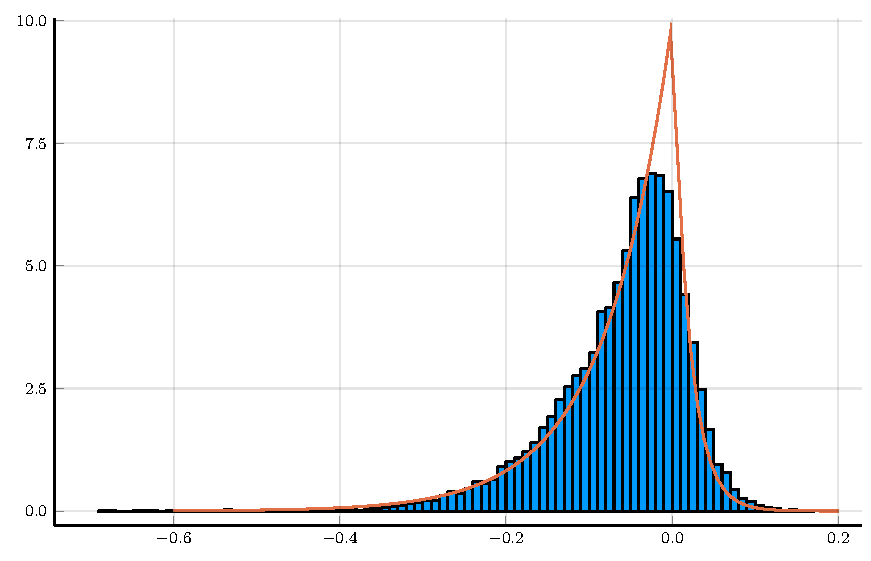
\includegraphics[width=0.49\textwidth]{media/boltzmannD01}}
  \subcaptionbox{$D=\frac{1}{5}$}{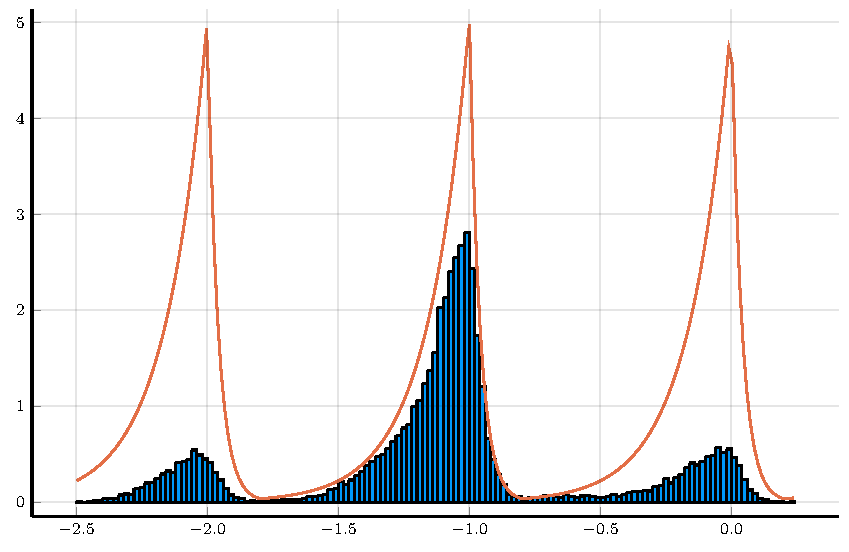
\includegraphics[width=0.49\textwidth]{media/boltzmannD02}}
  \caption{Simulated distribution, histogram, and the theoretical Boltzmann distribution, solid line, for $D=\frac{1}{10}$ and $D=\frac{1}{5}$.}
\end{figure}

\textbf{Task 8}

One should choose $\Delta U$ such that diffusion is maximized, without particles reaching over to neighbouring wells when the potential is on.
There will be three regimes of drift velocity, (1) too high frequency on the flashing will not allow the particles to diffuse enough, and we will see very little drift. (2) correct frequency will allow particles to diffuse beyond $\alpha$ and thus be trapped in the next well when the potential is turned on again. (3) the final regime will be a too large period, where particles will move both left and right, ie. they diffuse more than $1-\alpha$, and are trapped in wells in both directions.\\

We will now set $\Delta U = \SI{80}{\eV}$ and let $r = r_1$.


\textbf{Task 9}
With $D=\num{2E-4}$ simulating to $t=7000$ for different $\tau$, with 500 relizations for each $\tau$, the drift velocities shown in figure \ref{fig:drift_velocity} was found.
The drift velocity is here defined as the position in the final step.
From the figure one sees that the $\tau$ that optimizes drift velocity, $\tau_{opt}$ is 110.

Drift velocitites for $\tau = 100, 110, 120, 130, 140$ are 7.160835818693163, 7.174037267938745, 7.254817483579574, 7.297040033152324, 7.198623178831086.

Another simulation, with $\tau = 10, 30, 60, 80 100, 120$ gives 0.02214625656038857, 2.730464062719224, 6.089185824197861, 7.046632812276713, 7.463267755732644, 7.468415404324993.

\begin{figure}
  \centering
  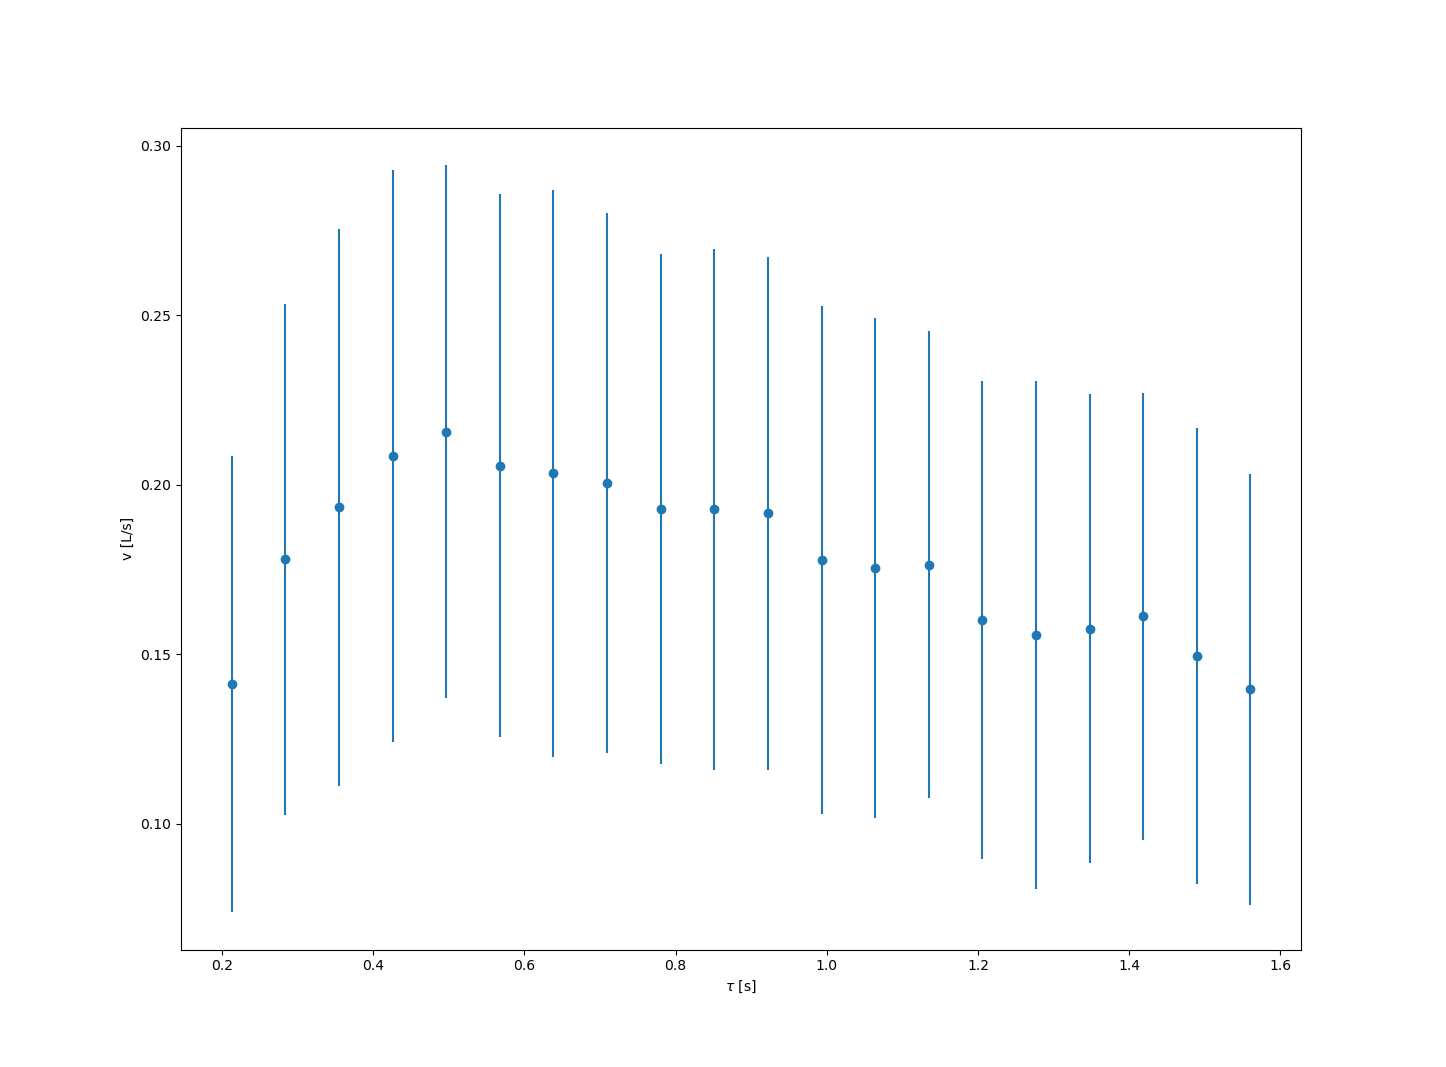
\includegraphics[width=.75\textwidth]{media/drift_velocity}
  \caption{Drift velocity for different flashing periods $\tau$.
    Calculated for $D=\num{2E-4}$ with $t_{\text{end}} = 7000$ and 500 relizations for each $\tau$.
    \label{fig:drift_velocity}}
\end{figure}


\textbf{Task 11}

We now consider a particle with radius $r_2 = 3r_1$.
Thus $\gamma_2 = 3\gamma_1$ and $\omega_2 = \frac{1}{3} \omega_1$.
Thus, this corresponds to scaling the time with a factor 3.

\textbf{Task 12}


\begin{figure}
  \centering
  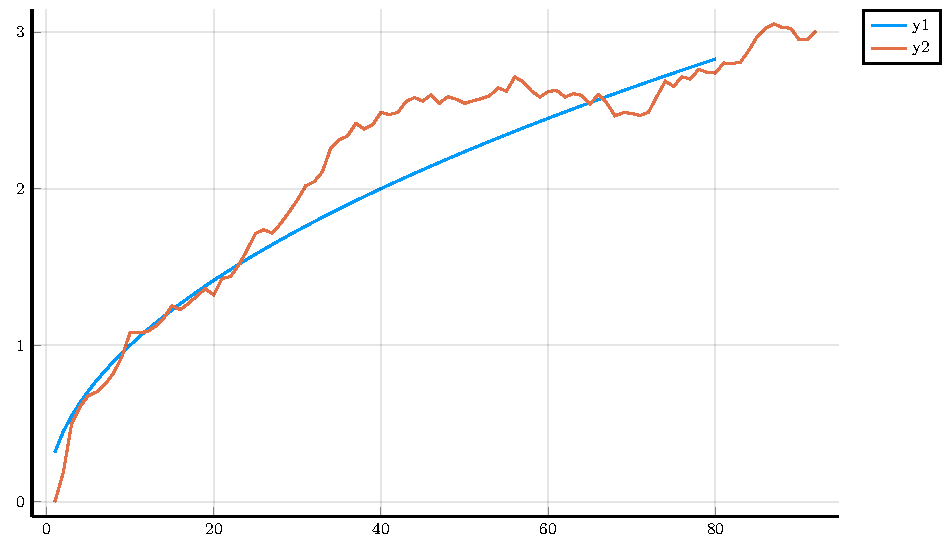
\includegraphics[width=.75\textwidth]{media/diffusion_std}
  \caption{Standard deviation of an ensable as a function of time. The solid line is a fit curve, which scales like $\sqrt{t}$, showing that the standard deviation behaves as expected.
  Calculated with $D = \num{2E-4}, t_{end} = 7000, \tau=110$.}

\end{figure}

\end{document}
